\documentclass[a4paper, 12pt]{article}
\usepackage[T2A]{fontenc} % кодировка
\usepackage[utf8]{inputenc} % кодировка исходного текста
\usepackage[english, russian]{babel} % локализация и переносы
\usepackage{graphicx} % Required for inserting images
\usepackage{cmap} % поиск в пдф
\usepackage{listings}
% \graphicspath{img/}

\usepackage{amsmath,amssymb,amsfonts,amsthm}
\theoremstyle{definition}
\newtheorem{definition}{Определение}

\usepackage{geometry}
\geometry{left=2.5cm}
\geometry{right=1.5cm}
\geometry{top=2.cm}
\geometry{bottom=2.cm}

\title{Отчет}
\author{Mikhail Safronov}
\date{October 2023}

\begin{document}
	
	% \maketitle
	
	\begin{titlepage}
		\begin{center}
			\large
			{МИНИСТЕРСТВО НАУКИ И ВЫСШЕГО ОБРАЗОВАНИЯ\\ РОССИЙСКОЙ ФЕДЕРАЦИИ}
			
			Федеральное государственное автономное образовательное учреждение высшего образования
			\vspace{0.5cm}
			
			\textbf{<<Национальный исследовательский Нижегородский государственный университет им. Н.И. Лобачевского>>}\\
			(ННГУ)\\
			\vspace{1cm}
			\textbf{Институт информационных технологий, математики и механики}\\
			\vspace{1cm}
			\textbf{Центр прикладных информационных технологий}
			%\textbf{Кафедра: Алгебры, геометрии и дискретной математики}
			\vspace{1cm}
			
			Направление подготовки: <<Фундоментальная информатика и информационные технологии>>\\
			Профиль подготовки: <<...>>
			\vfill
			
			
			
			\vfill
			
			\Large
			ЛАБОРАТОРНАЯ РАБОТА\\
			на тему:\\
			\textbf{<<Алгоритм Дейкстры на 3-куче и на 15-куче>>}
			{\LARGE 
			}
			\bigskip
			
			
		\end{center}
		\vfill
		
		\newlength{\ML}
		\settowidth{\ML}{«\underline{\hspace{0.7cm}}» \underline{\hspace{2cm}}}
		\hfill\begin{minipage}{0.4\textwidth}
			\textbf{Выполнил:}\\
			студент группы 3821Б1ФИ3\\
			Сафронов М. А.\\
		\end{minipage}%
		\bigskip
		
		\hfill\begin{minipage}{0.4\textwidth}
			\textbf{:}\\
			Преподаватель\\
			Уткин Г. В.\\
		\end{minipage}%
		\vfill
		
		\begin{center}
			Нижний Новгород\\
			2023 г.
		\end{center}
	\end{titlepage}
	
	\tableofcontents{}
	\clearpage
	
	\section{Введение}
	
	Поставлена задача "Алгоритм Дейкстры на троичной и пятнадцатиричной куче". Для того чтобы разобраться в этой теме, введем некоторые понятия, которые понадобяться в процессе выполнения. \newline
	
	Кучи - являются важными структурами данных, которые широко используются в области алгоритмов и программирования. \newline
	
	Алгоритм Дейкстры —
	это один из наиболее популярных алгоритмов, применяемых для поиска
	кратчайшего пути в графе. Комбинируя эти два концепта, мы получаем
	интересный подход: алгоритм Дейкстры, использующий 3-кучу и 15-
	кучу.\newline
	
	Одна из главных задач алгоритма Дейкстры заключается в нахождении
	кратчайшего пути между двумя узлами во взвешенном графе. Кратчайший
	путь определяется как путь с наименьшей суммой весов ребер. Алгоритм
	Дейкстры решает эту задачу путем осуществления пошагового обхода
	графа из начального узла и нахождения кратчайших путей до остальных
	узлов. \newline
	
	3-куча и 15-куча представляют собой
	особые варианты куч, которые дополнительно учитывают третий и пятнадцатый
	наименьшие элементы соответственно. Эти усовершенствованные кучи
	позволяют ускорить алгоритм Дейкстры, разработанный Эдсгером Дейкстрой,
	и сделать его более эффективным при работе с большими объемами
	данных. \newline
	
	Одна из главных особенностей использования куч в алгоритме Дейкстры
	заключается в оптимизации операций вставки нового элемента и удаления
	минимального элемента из кучи. Учитывая третий и пятнадцатый наименьшие
	элементы вместе с минимальным элементом, мы можем более эффективно
	оптимизировать выбор наименьшего пути в ходе выполнения алгоритма
	Дейкстры.\\ \\
	Изначально алгоритм Дейкстры разработан для работы с обычными
	кучами, однако использование 3-кучи и 15-кучи позволяет достичь еще
	более высокой производительности и эффективности при поиске кратчайшего
	пути в графе. \newline
	
	Таким образом, в данной лабораторной работе мы исследуем и реализуем
	алгоритм Дейкстры, используя 3-кучу и 15-кучу, и оценим
	
	\begin{definition}[Граф]
		Пусть $G=(V,E,W)$ - ориентированный граф без петель со взвешанными ребрами, где множество вершин $V = {(1,...,n)}$, множество ребер\\
		$E\in V*V,|E|=m$, и весовая  функция $W (u,v)$ каждому ребру $(u,v)\in E$ ставит в соответсвии его вес - неотрицательное число. Требуется найти кратчайшие пути от заданной вершины $s\in V$ до всех остальных вершин.
	\end{definition}
	Алгоритм Дейкстры работает только для графов без рёбер отрицательного веса.
	Сложность: $O(n^2)$ \newline
	
	Задача о кратчайших путях заключается в поиске кратчайшего пути между двумя вершинами в графе. Алгоритм Дейкстры - это один из алгоритмов, который позволяет решать эту задачу. Он работает следующим образом:
	
	\begin{enumerate}
		\item Начинаем с вершины, из которой нужно найти кратчайший путь.
		\item Для каждой смежной вершины вычисляем расстояние от начальной вершины до этой вершины.
		\item Если это расстояние меньше, чем уже известное расстояние до этой вершины, то обновляем значение расстояния.
		\item Повторяем шаги 2-3 для всех смежных вершин.
		\item Повторяем шаги 2-4 для всех вершин графа.
	\end{enumerate}
	\begin{definition}[Куча]
		Куча (или бинарная куча) --- это структура данных, которая представляет собой полное бинарное дерево, в которой каждый узел имеет значение, которое меньше или равно значению его потомков.
	\end{definition}
	\begin{definition}[3-Куча]
		Троичная куча --- это структура данных, которая представляет собой упорядоченное дерево с максимум тремя потомками, в которой каждый узел имеет значение, и значение в родительском узле меньше или равно значениям в его потомке
	\end{definition}
	\begin{definition}[15-Куча]
		Троичная куча --- это структура данных, которая представляет собой упорядоченное дерево с максимум пятнадцатью потомками, в которой каждый узел имеет значение, и значение в родительском узле меньше или равно значениям в его потомке
	\end{definition}
	В нашем случае мы будем использоваться: Троичную кучу и пятнадцатиричную кучу - это разновидности куч, которые отличаются от обычной кучи тем, что они имеют более сложную структуру. \newline
	
	Троичная куча позволяет хранить элементы в виде бинарного дерева, в котором каждый узел имеет три потомка. Пятнадцатиричная куча - это куча, в которой каждый узел имеет 15 потомков.Основное отличие между троичной кучей и обычной бинарной кучей заключается в том, что в троичной куче каждый узел имеет больше потомков, что позволяет уменьшить высоту дерева и ускорить операции вставки и удаления элементов. Кроме того, троичная куча может быть более эффективной, чем бинарная куча, когда требуется хранить большое количество элементов. \newline
	
	Однако, пятнадцатиричная куча не является стандартной структурой данных, и ее использование не распространено. Это связано с тем, что узлы с таким большим количеством потомков могут быть сложными для обработки и хранения, что может привести к увеличению времени выполнения операций вставки, удаления и поиска элементов.
	\newpage
	\section{Описание Класса и Алгоритмов}
	\subsection{TernaryHeap}
	\begin{verbatim}
		Переменные:
		- `heap`: Список, представляющий кучу.
		- `size`: Максимальный размер кучи.
		- `current.size`: Текущий размер кучи.
		
		Методы:
		- `push(value)`: Добавляет элемент `value` в кучу.
		Если куча уже заполнена, возвращает сообщение "Куча заполнена".
		- `pop()`: Извлекает и возвращает наименьший элемент из кучи.
		Если куча пуста, возвращает `None`.
		- `sift.up(index)`: Вспомогательный метод, который выполняет 
		восстановление свойств пирамиды (кучи) после добавления элемента в кучу.
		- `sift.down(index)`: Вспомогательный метод, который выполняет
		 восстановление свойств пирамиды (кучи) после удаления элемента из кучи.
	\end{verbatim}
	\subsection{Graph3}
	\begin{verbatim}
		Переменные:
		- `vertices`: Словарь, содержащий вершины графа и их смежные вершины.
		- `edges`: Словарь, содержащий ребра графа и их веса.
		
		Методы:
		- `add.vertex(vertex)`: Добавляет вершину `vertex` в граф.
		- `add.edge(source, destination, weight)`: Добавляет ребро с исходной
		 вершиной `source`, целевой вершиной `destination` и весом `weight`.
		- `dijkstra(source)`: Выполняет алгоритм Дейкстры для нахождения 
		кратчайших путей от вершины `source` до всех остальных вершин графа.
		 Возвращает словарь, содержащий вершины и их минимальные расстояния 
		 от исходной вершины.
		- `generate.graph(num.vertices, num.edges, weight.range, results.file)`:
		 Генерирует случайный граф с заданным количеством вершин `num.vertices` и
		  ребер `num.edges`, случайными весами ребер в диапазоне `weight.range` 
		  и записывает результаты выполнения алгоритма Дейкстры в файл `results.file`.
		- `draw.graph()`: Визуализирует граф с помощью библиотеки `networkx`
		и `matplotlib`.
		- `clear()`: Очищает граф, удаляя все вершины и ребра.
	\end{verbatim}
	\subsection{Описание алгоритма Дейкстры}
	
		Алгоритм начинает с инициализации расстояний до всех вершин как "бесконечность", кроме исходной вершины, которая инициализируется со значением 0. Затем, используя структуру данных "куча" (как, например, куча с тремя ветвями), мы поддерживаем актуальное расстояние для каждой вершины. \newline
		
		На каждой итерации алгоритма мы выбираем вершину с наименьшим текущим расстоянием и рассматриваем ее соседей. Для каждого соседнего узла мы вычисляем новое расстояние, которое будет равно сумме текущего расстояния до текущей вершины и веса ребра между текущей вершиной и соседним узлом.\newline
		
		Если новое расстояние меньше текущего расстояния до соседнего узла, мы обновляем расстояние до этого узла. Затем мы помещаем обновленное расстояние и соседний узел в кучу, чтобы поддерживать актуальность данных.\newline
		
		Процесс повторяется до тех пор, пока куча не будет пуста. По завершении выполнения алгоритма, для каждой вершины будет определено минимальное расстояние от исходной вершины, а также путь для достижения каждой вершины.\newline
		\subsection{Сложность Дейкстры}
		\begin{verbatim}
	def dijkstra(self, source):
  distance = {vertex: float('inf') for vertex in self.vertices}  # O(n)
  distance[source] = 0  # O(1)
  heap = TernaryHeap(len(self.vertices))  # O(n)
  for vertex in self.vertices:  # O(n)
      heap.push((distance[vertex], vertex))  # O(log n)
		
  while heap.current_size > 0:  # O(n)
      _, current_vertex = heap.pop()  # O(log n)
		
      for neighbor in self.vertices[current_vertex]:  # O(m)
          if current_vertex not in self.edges or neighbor not in
           self.edges[current_vertex]:  # O(1)
              print(f"Ошибка: вершины {current_vertex} и/или {neighbor}
              отсутствуют в списке смежности")  # O(1)
              continue
      new_distance = distance[current_vertex] +
      + self.edges[current_vertex][neighbor]  # O(1)
      if new_distance < distance[neighbor]:  # O(1)
          distance[neighbor] = new_distance  # O(1)
          heap.push((new_distance, neighbor))  # O(log n)
		
  return distance  # O(1)
			
		\end{verbatim}
	
	
	\section{Результаты}
	\subsection{Проверка алгоритма Дейкстры. Первый тест.} Сравнение алгоритма Дейкстры на троичной и пятнадцатиричной
	куче. Проверка коректности работы алгоритма дейкстры на малых данных.
	Создаем граф с 8-ю вершинами и с 11-ю ребрами.\\
	\begin{figure}[h]
		\centering
		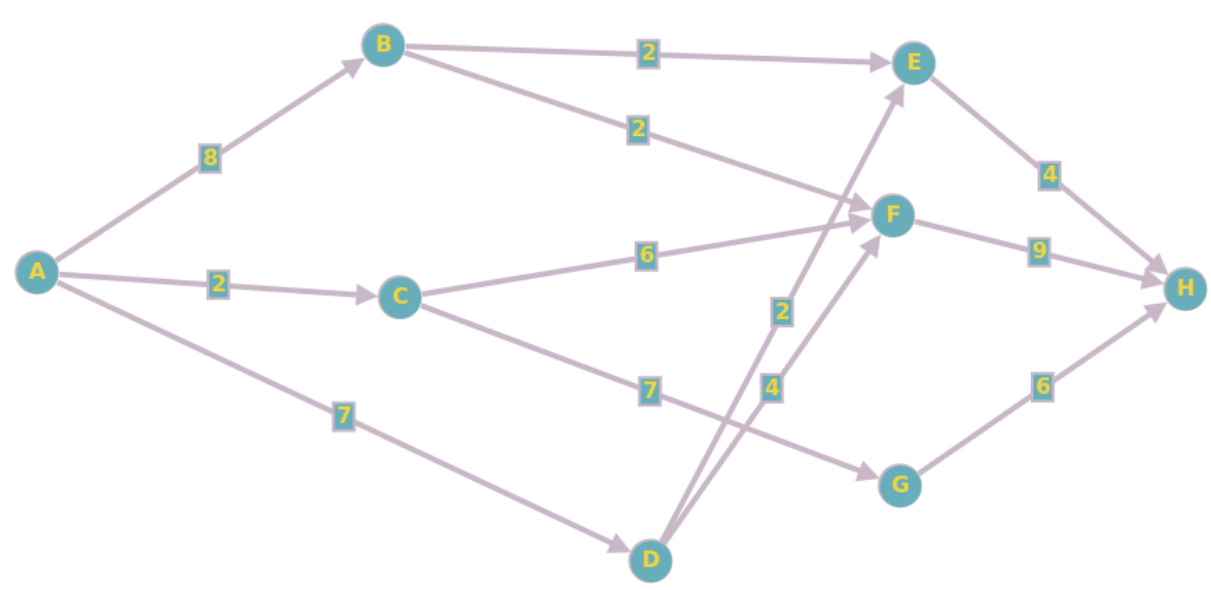
\includegraphics[scale=0.2]{img/1graph.png}
		\caption{Граф из первого теста}
	\end{figure}
	\begin{verbatim}
		Результат работы программы:
		{'A': 0, 'B': 8, 'C': 2, 'D': 7, 'F': 8, 'G': 9, 'E': 9, 'H': 13}
	\end{verbatim}
	Не трудно заметить, что вывод верный и действительно вес кратчайшего
	пути от A до H составляет 13.\\ \\
	\newpage
	\subsection{Проверка алгоритма Дейкстры. Второй тест}
	Похож на предыдущий только немного больше данных, для того
	чтобы убедиться в корректности алгоритма.\newline
	\begin{figure}[h]
		\centering
		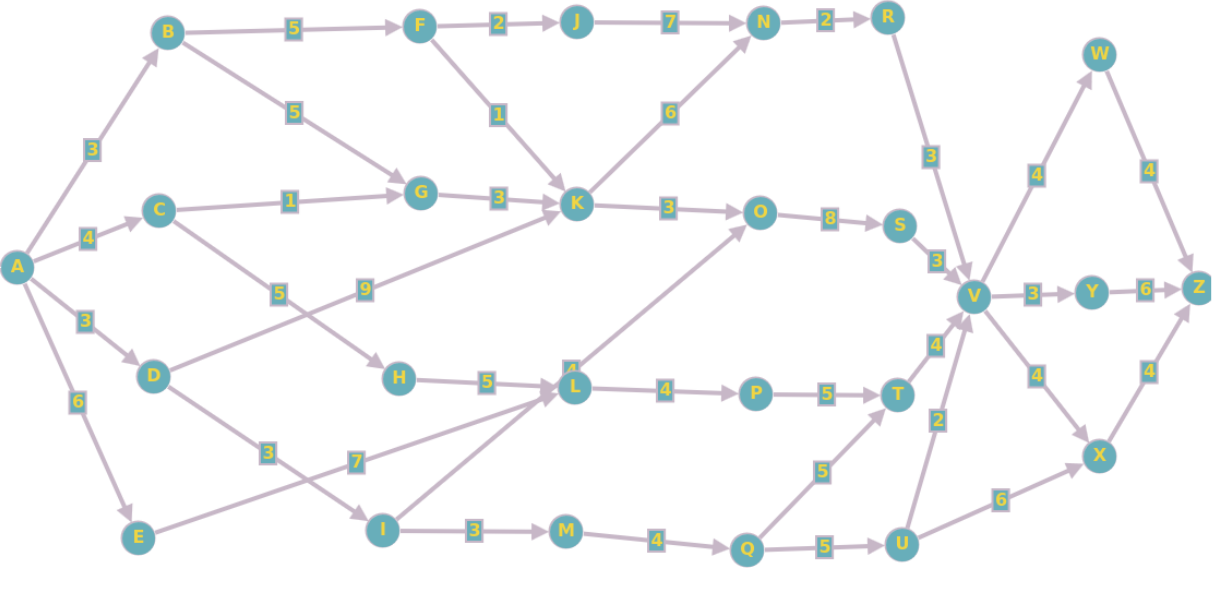
\includegraphics[scale=0.2]{img/2graph.png}
		\caption{Граф из второго теста}
		\label{fig:my_image}
	\end{figure}
	На картинке 1.2 можно увидеть граф с большим количеством вершин и
	ребер, чем на предыдущем примере. Применив алгоритм Дейкстры для
	графа на 3-куче и 15-куче получим следующий вывод.
	\begin{verbatim}
		Результат работы программы:
		{'A': 0, 'B': 3, 'C': 4, 'D': 3, 'E': 6, 'F': 8, 'G': 5, 'K': 8, 'I': 6,
			 'H': 9, 'L': 13, 'O': 10, 'M': 9, 'J': 10, 'N': 14, 'Q': 13, 'S': 18, 
			 'P': 17, 'T': 18, 'U': 18, 'R': 16, 'V': 19, 'X': 23,
			  'W': 23, 'Y': 22, 'Z': 27}
	\end{verbatim}
	Отсюда делаем вывод, что алгоритм Дейкстры так-же работает корректно и теперь займемся временем работы алгоритма, в данном примере алгоритм на 3-куче лидирует по времени.\newline
	\subsection{Тестирование на различных входных данных}
	\subsubsection{Первый тест а}
	Количество вершин: $n = 1, ... , 10^4+1$ \newline
	Шаг = 250 \newline
	Нижняя граница для мощности ребер: $q = 1$ \newline
	Верхняя границы для мощности ребер: $r = 10^6$ \newline
	Количество ребер: m = $n^2/10$ \newline
	\begin{figure}[!ht]
		\centering
		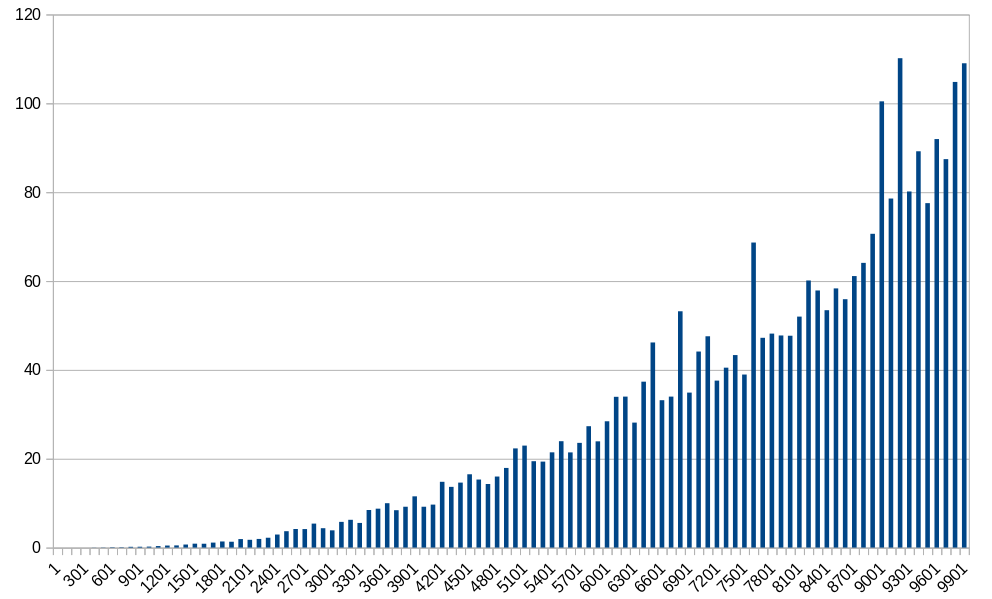
\includegraphics[width=1\textwidth]{img/res1a_3.png}
		\caption{График зависимости входных данных от веремени алгоритма Дейкстры на 3-куче теста 1а}
		\label{fig:my_image}
	\end{figure}
	
	\begin{figure}[!ht]
		\centering
		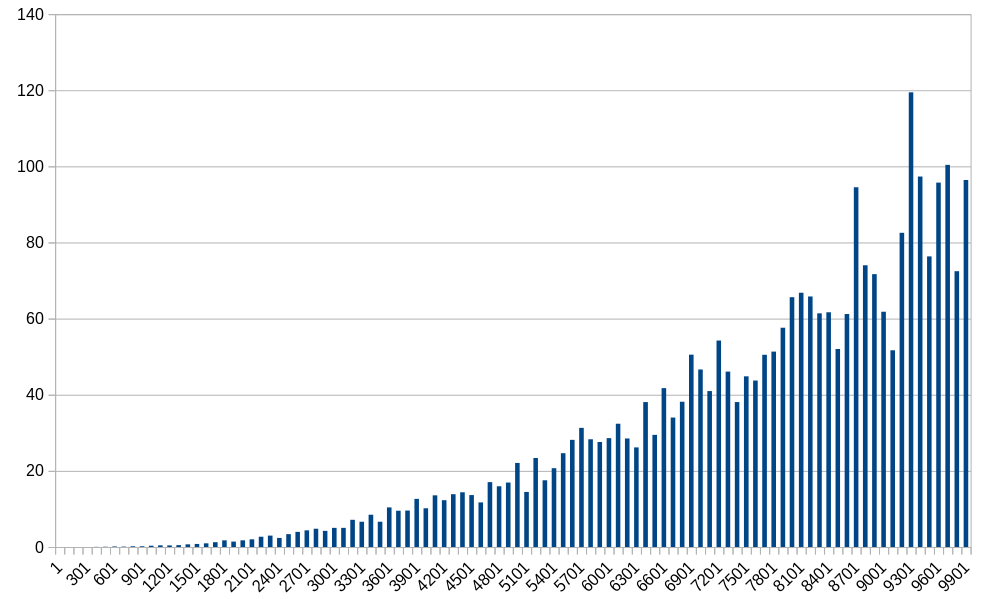
\includegraphics[width=1\textwidth]{img/res1a_15.png}
		\caption{График зависимости входных данных от веремени алгоритма Дейктсры на 15-куче теста 1а}
		\label{fig:my_image}
	\end{figure}
	\newpage
	
	\subsubsection{Первый тест б}
	Количество вершин: $n = 1, ... , 10^4+1$ \newline
	Шаг = 250 \newline
	Нижняя граница для мощности ребер: $q = 1$ \newline
	Верхняя границы для мощности ребер: $r = 10^6$ \newline
	Количество ребер: m = $n^2$ \newline
	
	\begin{figure}[!ht]
		\centering
		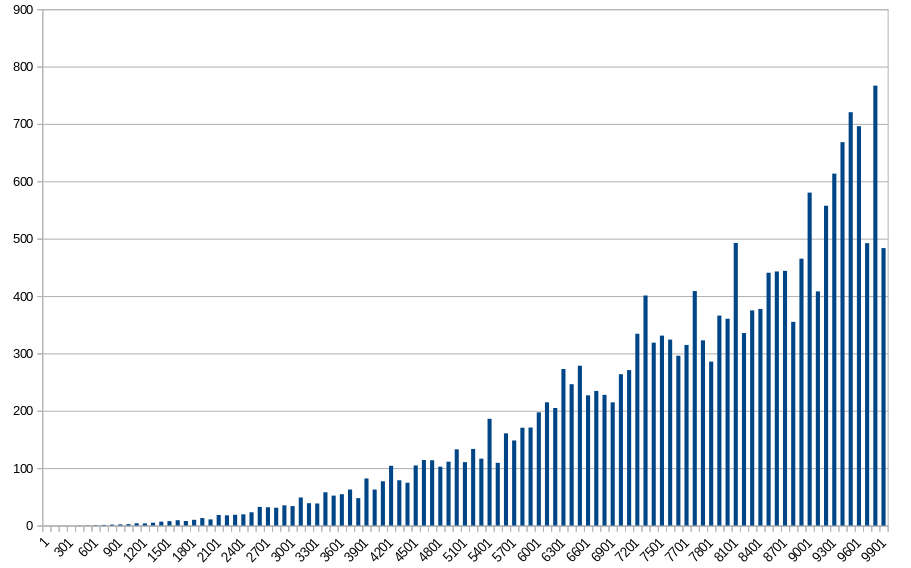
\includegraphics[width=1\textwidth]{img/res1b_15.png}
		\caption{График зависимости входных данных от веремени алгоритма Дейктсры на 3-куче теста 1b}
		\label{fig:my_image}
	\end{figure}
	
	\begin{figure}[!ht]
		\centering
		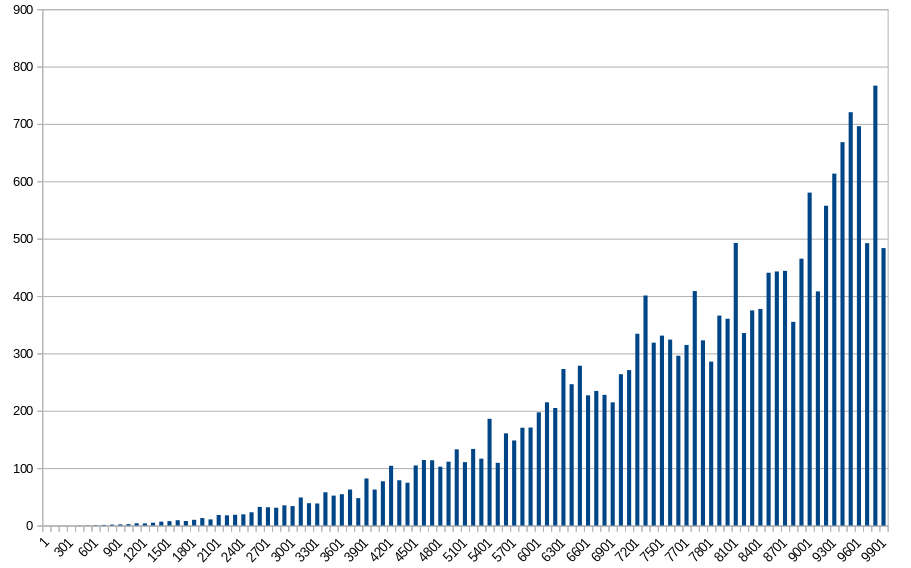
\includegraphics[width=1\textwidth]{img/res1b_15.png}
		\caption{График зависимости входных данных от веремени алгоритма Дейктсры на 15-куче теста 1b}
		\label{fig:my_image}
	\end{figure}
	\newpage
	
	\subsubsection{Второй тест а}
	Количество вершин: $n = 1, ... , 10^4+1$ \newline
	Шаг = 100 \newline
	Нижняя граница для мощности ребер: $q = 1$ \newline
	Верхняя границы для мощности ребер: $r = 10^6$ \newline
	Количество ребер: m = $100*n$ \newline
	
	\begin{figure}[!ht]
		\centering
		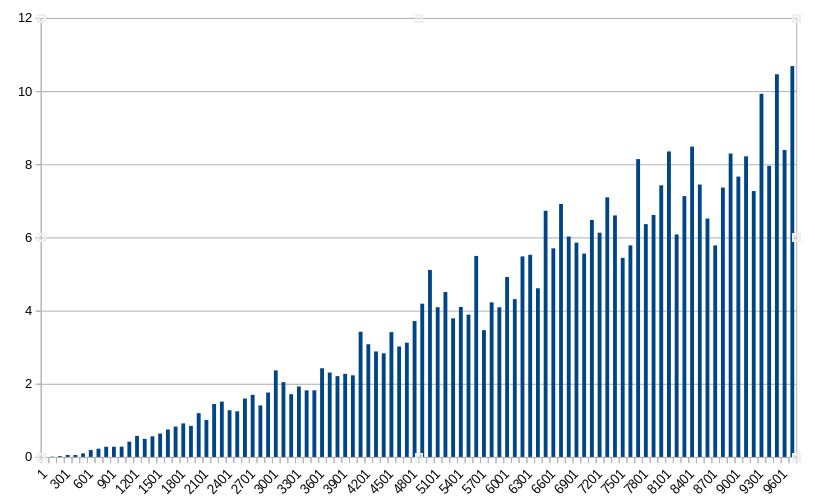
\includegraphics[width=1\textwidth]{img/res2a_3.png}
		\caption{График зависимости входных данных от веремени алгоритма Дейкстры на 3-куче теста 2а}
		\label{fig:my_image}
	\end{figure}
	
	\begin{figure}[!ht]
		\centering
		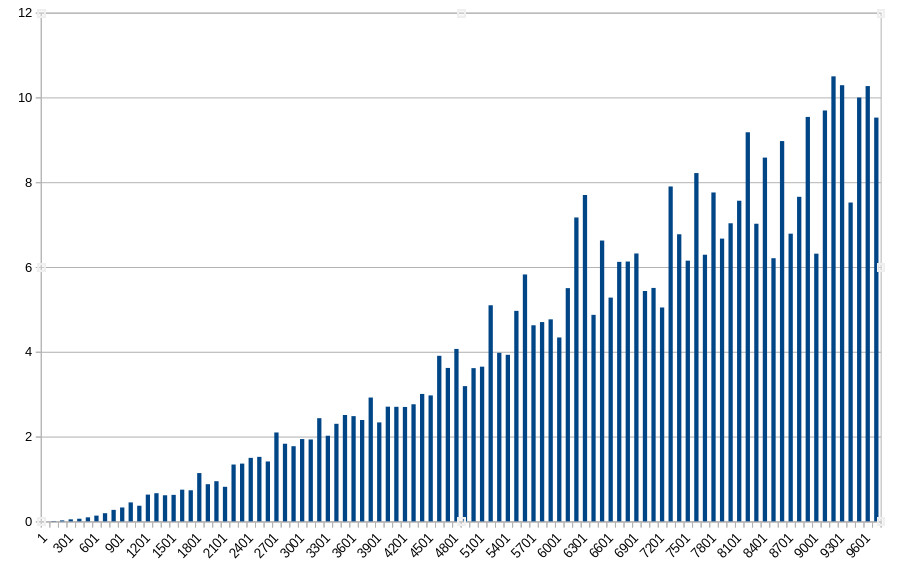
\includegraphics[width=1\textwidth]{img/res2a_15.png}
		\caption{График зависимости входных данных от веремени алгоритма Дейкстры на 15-куче теста 2а}
		\label{fig:my_image}
	\end{figure}
	
	\newpage
	
	\subsubsection{Второй тест б}
	
	Количество вершин: $n = 1, ... , 10^4+1$ \newline
	Шаг = 100 \newline
	Нижняя граница для мощности ребер: $q = 1$ \newline
	Верхняя границы для мощности ребер: $r = 10^6$ \newline
	Количество ребер: m = $1000*n$ \newline
	
	\begin{figure}[!ht]
		\centering
		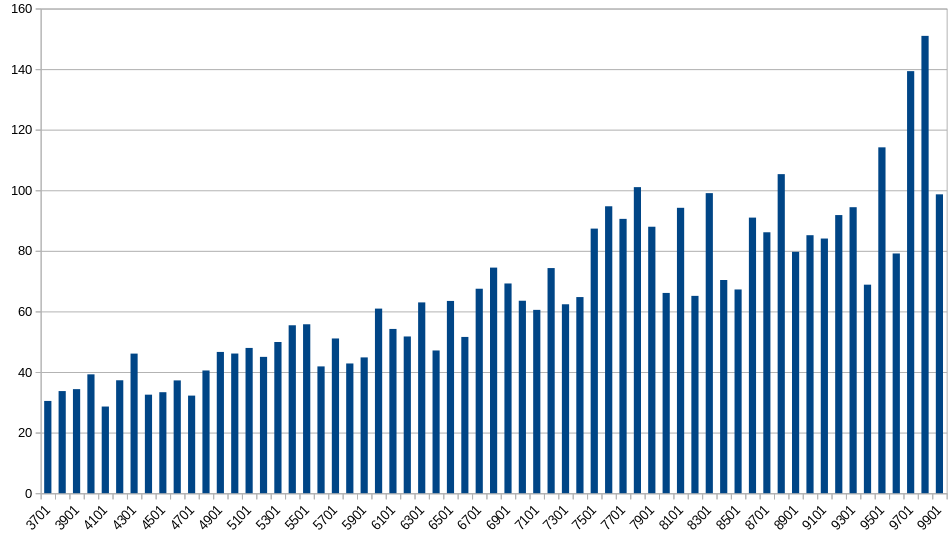
\includegraphics[width=1\textwidth]{img/res2b_3.png}
		\caption{График зависимости входных данных от веремени алгоритма Дейкстры на 3-куче теста 2b}
		\label{fig:my_image}
	\end{figure}
	
	\begin{figure}[!ht]
		\centering
		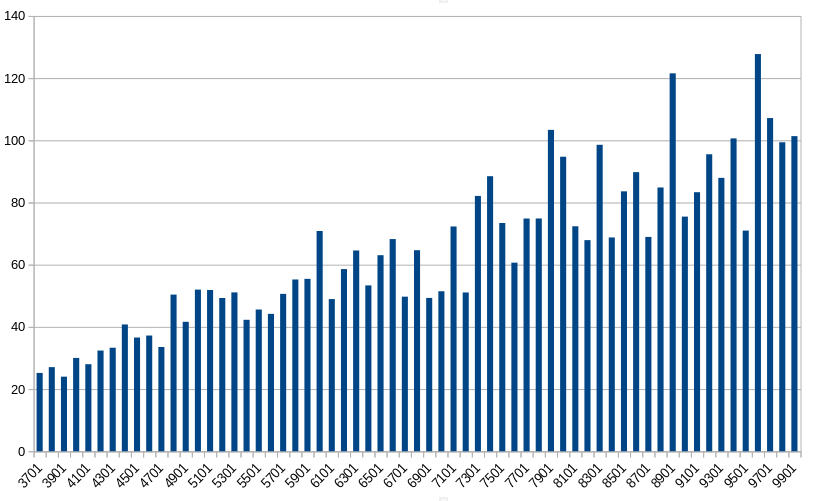
\includegraphics[width=1\textwidth]{img/res2b_15.png}
		\caption{График зависимости входных данных от веремени алгоритма Дейкстры на 15-куче теста 2b}
		\label{fig:my_image}
	\end{figure}
	\newpage
	
	\subsubsection{Третий тест}
	Количество вершин: $n = 10^4+1$ \newline
	Нижняя граница для мощности ребер: $q = 1$ \newline
	Верхняя границы для мощности ребер: $r = 10^6$ \newline
	Количество ребер: m = $0,...,10^7$ \newline
	Шаг = $10^5$ \newline
	
	\begin{figure}[!ht]
		\centering
		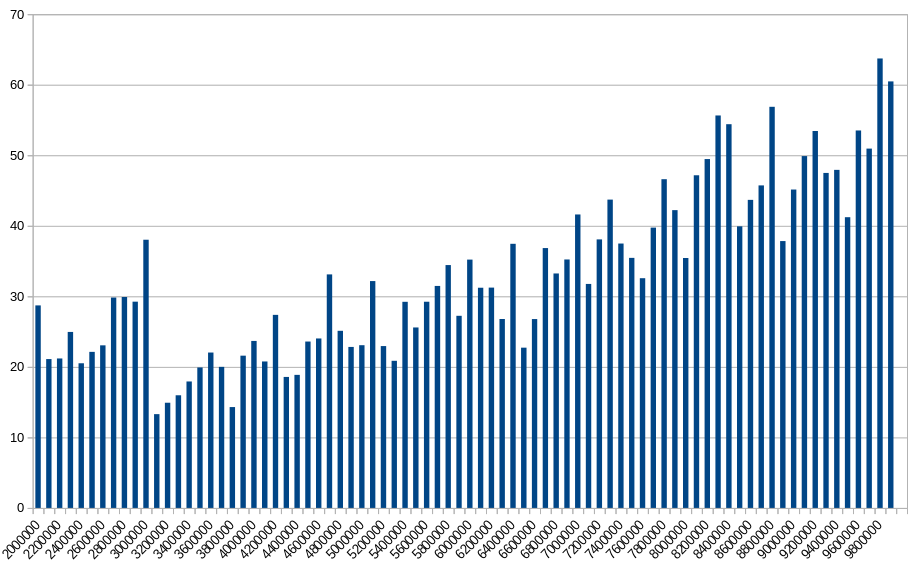
\includegraphics[width=1\textwidth]{img/res3_3.png}
		\caption{График зависимости входных данных от веремени алгоритма Дейкстры на 3-куче теста 3}
		\label{fig:my_image}
	\end{figure}
	
	\begin{figure}[!ht]
		\centering
		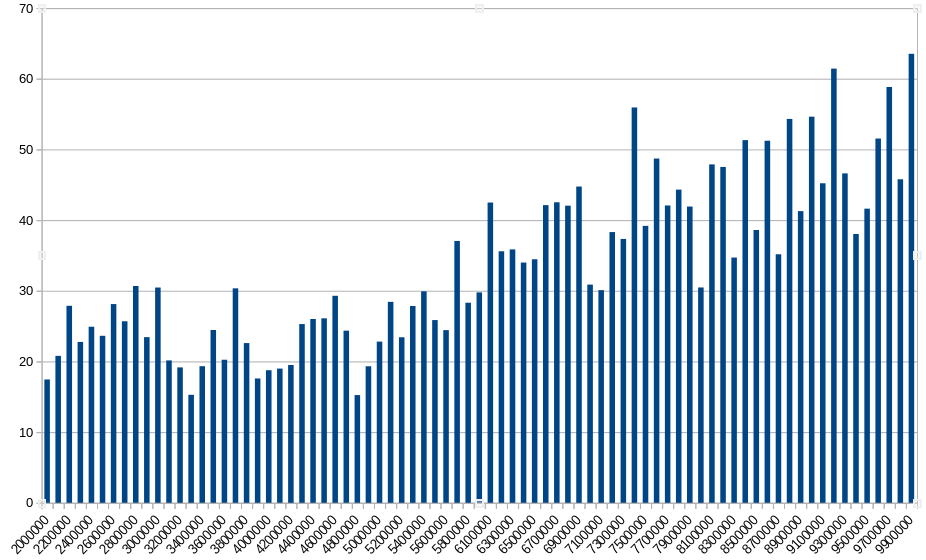
\includegraphics[width=1\textwidth]{img/res3_15.png}
		\caption{График зависимости входных данных от веремени алгоритма Дейкстры на 15-куче теста 3}
		\label{fig:my_image}
	\end{figure}
	
	\newpage
	
	\subsubsection{Четвертый тест а}
	
	Количество вершин: $n = 10^4+1$ \newline
	Нижняя граница для мощности ребер: $q = 1$ \newline
	Верхняя границы для мощности ребер: $r = 1,...,200$ \newline
	Шаг = 1 \newline
	Количество ребер: m = $n^2$ \newline
	
	\begin{figure}[!ht]
		\centering
		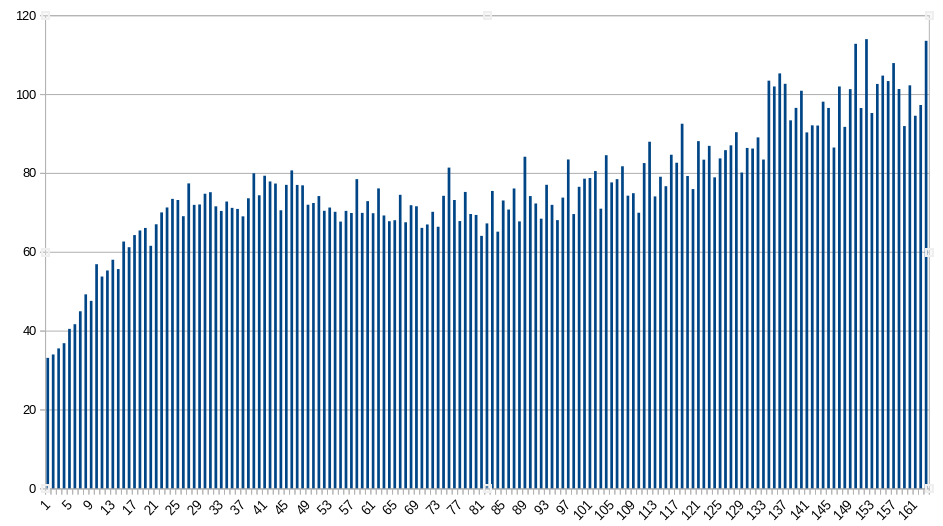
\includegraphics[width=1\textwidth]{img/res4a_3.png}
		\caption{График зависимости входных данных от веремени алгоритма Дейкстры на 3-куче теста 4а}
		\label{fig:my_image}
	\end{figure}
	
	\begin{figure}[!ht]
		\centering
		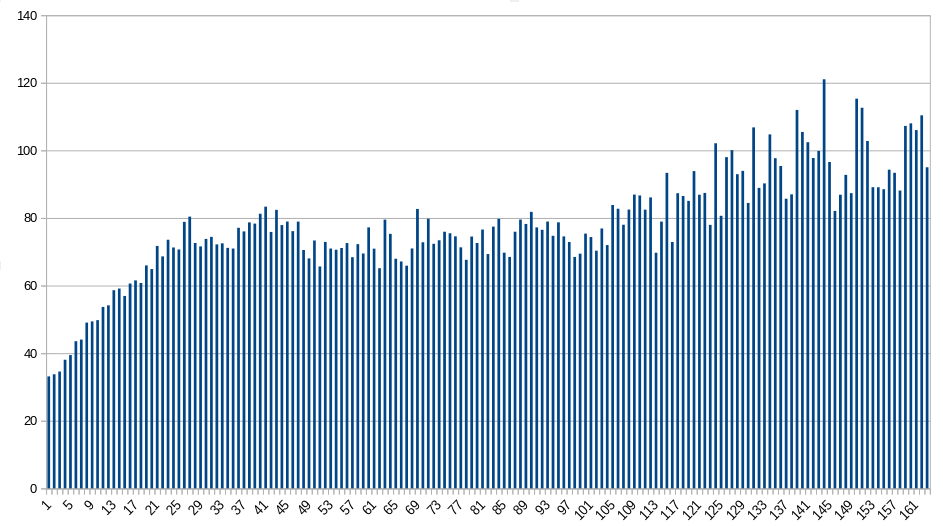
\includegraphics[width=1\textwidth]{img/res4a_15.png}
		\caption{График зависимости входных данных от веремени алгоритма Дейкстры на 15-куче теста 4а}
		\label{fig:my_image}
	\end{figure}
	\newpage
	
	\subsubsection{Четвертый тест б}
	Количество вершин: $n = 10^4+1$ \newline
	Нижняя граница для мощности ребер: $q = 1$ \newline
	Верхняя границы для мощности ребер: $r = 1,...,200$ \newline
	Шаг = 1 \newline
	Количество ребер: m = $1000*n$
	\begin{figure}[!ht]
		\centering
		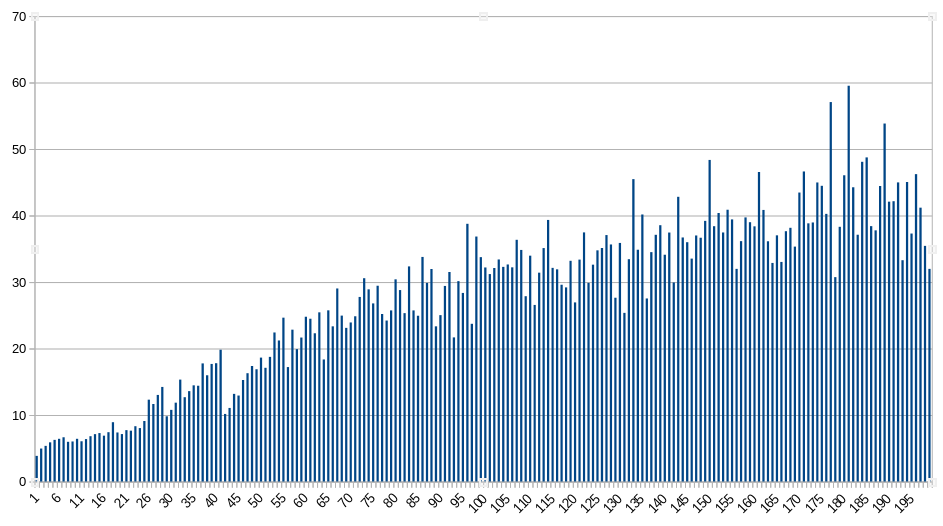
\includegraphics[width=1\textwidth]{img/res4b_3.png}
		\caption{График зависимости входных данных от веремени алгоритма Дейкстры на 3-куче теста 4b}
		\label{fig:my_image}
	\end{figure}
	
	\begin{figure}[!ht]
		\centering
		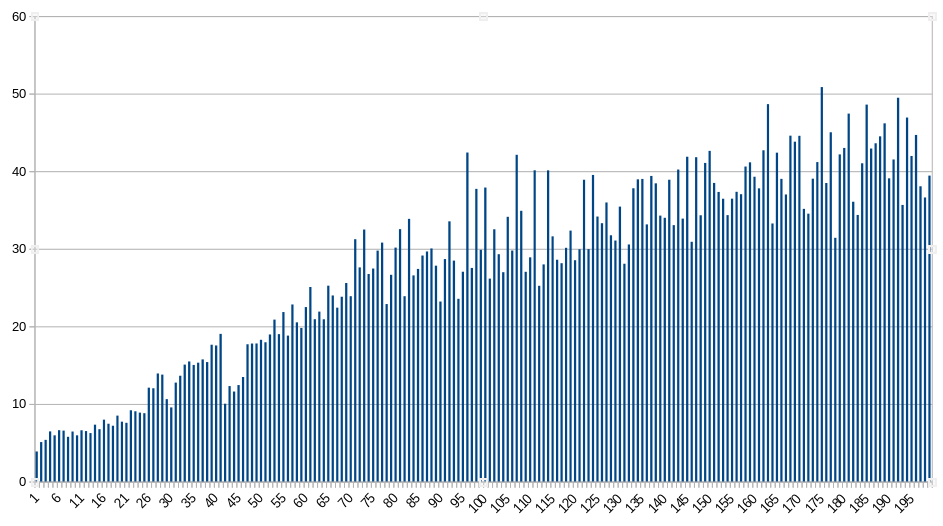
\includegraphics[width=1\textwidth]{img/res4b_15.png}
		\caption{График зависимости входных данных от веремени алгоритма Дейкстры на 15-куче теста 4b}
		\label{fig:my_image}
	\end{figure}
	
	\clearpage
	\subsection{Конфигурация компьютера}
	\begin{verbatim}
		OS: Windows 10
		CPU: Ryzen 5 3600
		RAM: 16gb 3200 

	\end{verbatim}
	
	\section{Вывод}
	В ходе выполнения лабораторной работы удалось достич следующих целей
	\begin{itemize}
		\item Разобраться в понятих 3-куча, 15-куча, понять их различия.
		\item Реализовать классы куч и класса Граф.
		\item Проверить корректную работу алгоритма Дейкстры в нескольких тестах.
		\item Исследовать отличия алгоритма Дейкстры на 3-куче и 15-куче.
		
	\end{itemize}
	
	Так как алгоритм Дейкстры решает немалую долю задач в жизни человека, то исходя из тестов, найдутся такие задачи в которых алгоритм на 15-куче будет быстрее находить кратчайшие пути, а значит будет использоваться в решение задач, нужно лишь тщательно проанализировать и выбрать наиболее прагматичный вариант для конкретной задачи.
	
\end{document}
